\usetikzlibrary{arrows.meta,calc}
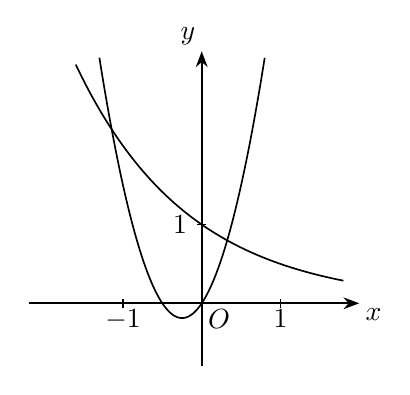
\begin{tikzpicture}[x=1cm,y=1cm,line width=.6pt,>=Stealth,font=\normalsize]
% Axes: x to 2.0 (last tick 1 + half grid), y to 3.2
\draw[->] (-2.200000,0) -- (2.000000,0);
\node[anchor=west,inner sep=0pt,xshift=2.000000pt,yshift=-4.000000pt] at (2.000000,0) {$x$};
\draw[->] (0,-0.800000) -- (0,3.200000);
\node[anchor=south,inner sep=0pt,xshift=-5.000000pt,yshift=2.000000pt] at (0,3.200000) {$y$};
% x ticks at -1, 1
\draw ( -1.000000,0.060000) -- (-1.000000,-0.060000);
\node[anchor=north,inner sep=0pt,yshift=-2.000000pt] at (-1.000000,0) {$-1$};
\draw (1.000000,0.060000) -- (1.000000,-0.060000);
\node[anchor=north,inner sep=0pt,yshift=-2.000000pt] at (1.000000,0) {$1$};
\node[below right,inner sep=0pt,xshift=2pt,yshift=-2pt] at (0,0) {$O$};
% y=1 tick + label (exponential passes (0,1)); label offset left to clear stroke
\draw (0.060000,1.000000) -- (-0.060000,1.000000);
\node[anchor=east,inner sep=0pt,xshift=-5.000000pt] at (0,1.000000) {$1$};

% Parabola representative: y=x^2+0.5x, zeros 0,-0.5, opening up
\draw[domain=-1.300000:0.800000,samples=101,smooth] plot (\x,{3*\x*\x+1.5*\x});
% Exponential representative: y=0.5^x decreasing through (0,1)
\draw[domain=-1.600000:1.800000,samples=101,smooth] plot (\x,{pow(0.5,\x)});
\end{tikzpicture}
